	Acerca do projeto da bancada de testes não destrutivos para amortecedores de carros populares,descreve-se a seguir as definições de projeto da área de eletrônica.

	\textbf{Objetivo}

	Desenvolver a central de controle da bancada e sensoreamento de parâmetros do projeto.

	\textbf{EAP}

	Na EAP do projeto eletrônico, mostrada na Figura \ref{EAPeletronica}, apresenta-se o detalhamento dos pacotes de trabalho e os entregáveis definidos para o desenvolvimento do projeto eletrônico.

	\begin{figure}[!h]
		\centering
		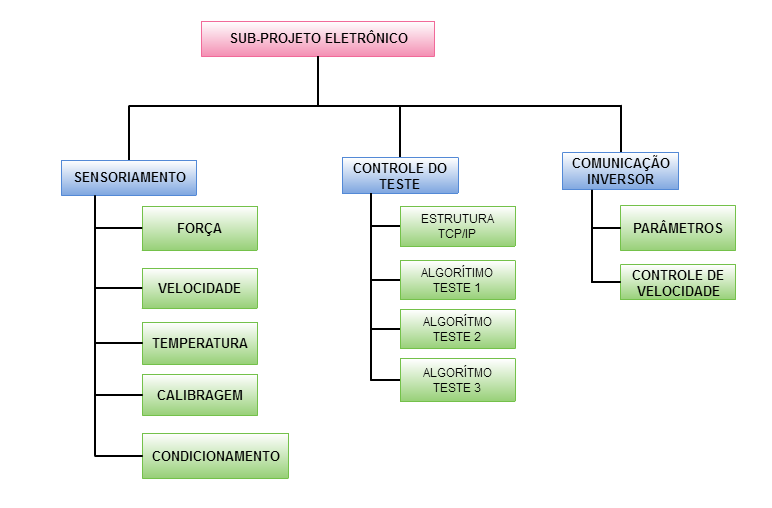
\includegraphics[scale=0.6]{EAPeletronica.png}
		\caption{Estrutura Analítica do Projeto Eletrônico}
		\label{EAPeletronica}
	\end{figure}


	Nos parágrafos a seguir descreve-se brevemente os pacotes de trabalho apresentados na EAP do projeto eletrônico. 

	\textit{Sensoriamento}: Corresponde ao sistema responsável por realizar a aquisição dos dados referente à temperatura do amortecedor, à força de reação do amortecedor e a velocidade da haste. O desenvolvimento de rotinas de calibração e a construção do circuito de condicionamento desses sinais também estão compreendidos nesse pacote de trabalho.

	\textit{Controle do Teste}: Esse ramo da EAP corresponde ao desenvolvimento dos algorítmos de controle de execução dos testes a partir dos dados recebidos, através de protocolo TCP/IP, informados pelo usuário. 

	\textit{Comunicação com o inversor}: Esse ramo compreende ao interfaceamento entre a sída da BBB e a entrada analógica do inversor, logo aspectos como a parametrização e a configuração do inversor também estão incluídos.

	\textbf{Lista É / Não É}

	\textit{ É função da equipe do projeto eletrônico:}

	\begin{itemize}

		\item Selecionar os sensores, dada as especificações exigidas pelo projeto, que devem ser obtidas dos subgrupos da área de Mecânica e Elétrica.
		\item Interfacear os sensores com a central, usando a plataforma da própria BBB.
		\item Desenvolver o sistema de comunicação da central usando um sistema linux. A central deverá estabelecer a comunicação (servidor e cliente) usando o protocolo TCP/IP.
		\item Controlar o motor AC trifásico, interfaceando o inversor com a BBB.
		\item Salvar os resultados em uma EEPROM.
		\item Prototipar uma placa de circuito impresso para o interfaceamento físico entre os sensores e a BBB.
		\item Desenvolver algorítmo de controle de execução do teste.

	\end{itemize}

	\textit{ Não é função da equipe do projeto eletrônico:}

	\begin{itemize}

		\item Desenvolver o sistema elétrico de acionamento da bancada.
		\item Desenvolver a fonte de conversão de 220AC para 5V DC.
		\item Desenvolver a interface gráfica para acionamento remoto (usando o cliente) da bancada.
		\item Definir quaisquer variáveis acerca do projeto mecânico, amortecedor e temperatura.

	\end{itemize}

	\textbf{Requisitos}

	Dada as definições de testes que serão executados na bancada, o sistema eletrônico deverá ser capaz de obter os parâmetros exigidos, tais como temperatura do amortecedor, velocidade linear da haste e força de reação do amortecedor; além disso, o sistema deverá ser desenvolvido com o protocolo TCP/IP, para permitir que seja desenvolvida a interface gráfica que irá controlar a bancada remotamente. O resultado deverá ser salvo em um sistema não volátil, para assegurar que caso ocorra alguma falha energética, os mesmos não se percam. Os sensores devem ser dimensionados de modo a satisfazer as condições de operação do teste. 

	\textbf{Propósito}

	Para a realização dos testes no amortecedor, existe a necessidade de obter parâmetros para a validação da especificação teórica, no que se refere a funcionalidade do amortecedor. Com isso, é necessário o desenvolvimento de um sistema que controle tanto as obtenções dos parâmetros exigidos, quanto o controle do teste e armazenamento dos resultados.

	\textbf{Stakeholders}

	Os integrantes Eduardo e Regina compõem a equipe de desenvolvimento eletrônico e estão diretamente relacionados. As equipes do desenvolvimento da aplicação web, formada pelos estudantes de engenharia de software, e a equipe de especificação e controle do motor, formada pelos estudantes de engenharia de energia, também estão envolvidos no projeto por haver pontos importantes de interação no processo de desenvolvimento.

	\textbf{Espectativa dos Stakeholders}

	Segundo a Figura \ref{EAPeletronica} mostra, tem-se a expectativa de entregar para o segundo ponto de controle a PCI de condicionamento, estrutura preliminar do algorítimo de controle dos testes, estrutura TCP/IP, algorítmo de aquisição dos dados de força, algorítmo de aquisição dos dados de proximidade.
	Para o terceiro ponto de controle espera-se entregaro sistema de controle de testes, os algorítmos de aquisição dos dados de temperatura, parametrização do inversor e implementação das rotinas de calibragem.

	\textbf{Cronograma}

	A Tabela \ref{cronogramaeletronica} mostra o cronograma desenvolvido em termos das macros do projeto eletrônico.

	\begin{table}[!h]
	\centering
	\caption{Cronograma de macros do projeto eletrônico}
	%\vspace{0.5cm}
	\begin{tabular}{ l c c }
	\hline
	\textbf{ATIVIDADE}	&	\textbf{DATA DE INÍCIO/FIM} &	\textbf{\% COMPLETO}\\
	\hline
	Definição da plataforma de controle		&	11/04 - 15/04  & 100\% \\
	\hline
	Definição dos sensores					&	15/04 - 25/04  & 100\% \\
	\hline
	Compra dos sensores						&	26/04 - 06/05  & 100\% \\
	\hline
	PCI de condicionamento					&	09/05 - 18/05  & 100\% \\
	\hline
	Estrutura TCP/IP						&	12/05 - 23/05  & 100\% \\
	\hline
	Aquisição dos dados de força			&	16/05 - 23/05  & 100\% \\
	\hline
	Aquisição dos dados de velocidade		&	19/05 - 01/06  & 100\% \\
	\hline
	Aquisição dos dados de temperatura		&	27/05 - 08/06  & 100\% \\
	\hline
	Controle do teste						&	27/05 - 13/06  & 100\% \\
	\hline
	Interfaceamento BBB com o inversor		&	13/06 - 16/06  & 100\% \\
	\hline
	Calibragem								&	16/06 - 23/06  & 100\% \\
	\hline

	\label{cronogramaeletronica}
	\end{tabular}
	\end{table}

	A Figura \ref{gantt} apresenta o Gráfico de Gantt desenvolvido para a execução das tarefas para o segundo e terceiro ponto de controle em conformidade com as espectativas do stakeholders.
	\newpage
	\begin{figure}[!h]
		\centering
		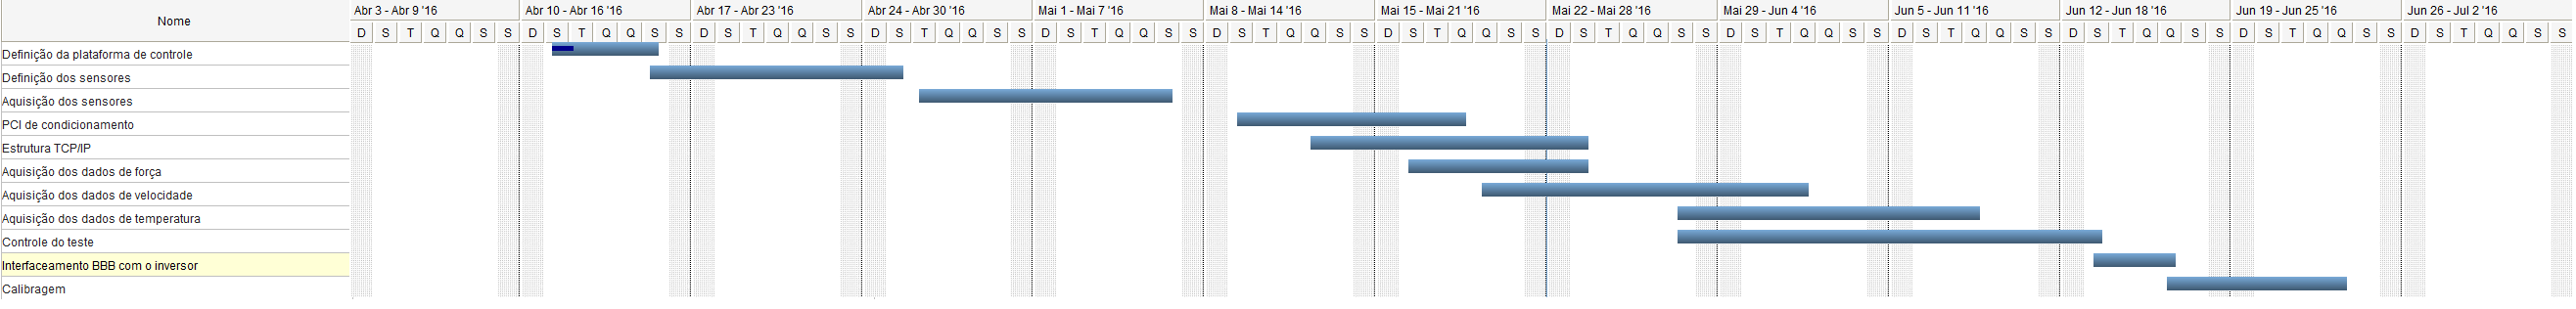
\includegraphics[scale=0.25]{gantt.png}
		\caption{Gráfico de Gantt do projeto eletrônico}
		\label{gantt}
	\end{figure}

	\textbf{Premissas}

	Para a execução do projeto eletrônico da bancada, considera-se verdadeiro as seguintes situações:
	\begin{itemize}

		\item As definições mecânicas estão bem definidas e não sofrerão alterações. O conjunto de sensores irão, além de captar dados importantes para as conclusões do teste do amortecedor, ser responsáveis pelo funcionamento da bancada. O dispositivo eletrônico, em nível de programação, ou seja, o controle da bancada por meio do sistema cliente/servidor, dado as informações capturadas pelos sensores requer a funcionalidade bem definida.
		\item O inversor de frequência, usado para controlar o motor elétrico, é compatível com o hardware (placa beaglebone). Isso permitirá o pleno controle por meio do sistema operacional embarcado.
		Dada as especificações de quais parâmetros devem ser adquiridos, os sensores necessários para tal tarefa devem estar disponíveis dentro do prazo definido para a etapa de instanciar os sensores no hardware e software escolhidos.
		\item O sistema embarcado deve atender a necessidade do projeto. Isso significa que todos os dados dos sensores devem obtidos, gravados e transmitidos para o cliente, que em nível de protótipo (no terminal) deve ser desenvolvido pela equipe de eletrônica e em nível de produto final será desenvolvido pela equipe de software.
		\item As definições elétricas, ou seja, alimentação do sistema eletrônico e de toda a bancada, devem ser desenvolvidos. Os circuitos necessários e placas de circuito impresso devem ser projetadas, testadas e instaladas no projeto.

	\end{itemize}

	\textbf{Restrições Organizacionais}

	Em virtude da divisão do grupo em equipes de desenvolvimento em função da sua áreas de formação e atuação no projeto, assim como a quantidade de integrantes que cursam engenharia eletrônica, o presente projeto possui pouca versatilidade para a equipe do projeto eletrônico, logo a equipe de desenvolvimento do projeto eletrônico não foi subdividida.

	\textbf{Investimento}

	A tabela \ref{investimentoeletronica} apresenta uma descrição preliminar do investimento projetado ao longo do projeto para aquisição de componentes eletrônicos.

	\begin{table}[!h]
	\centering
	\caption{Investimento do Projeto Eletrônico}
	\vspace{0.5cm}
	\begin{tabular}{ c c}
	\hline
	\textbf{DESCRIÇÃO}	&	\textbf{VALOR (R\$)}\\
	\hline
	Célula de Carga & 506,26 \\
	\hline
	MLX90614 & 155,00\\
	\hline
	BBB & 0,00\\
	\hline
	HC-SR04 & 0,00\\
	\hline
	Componentes Diversos & 30,00\\
	\hline
	\textbf{TOTAL} & \textbf{691,26}\\
	\hline

	\label{investimentoeletronica}
	\end{tabular}
	\end{table}

	\textbf{Riscos}

	Acerca do sistema eletrônico, tem-se os seguintes riscos:
	\begin{itemize}

		\item Quebra de um dos sensores: Isso resultará em atrasos, dado que os sensores foram comprados de outra cidade e tem-se o prazo de entrega envolvido no processo de aquisição. Além disso, os custos do projeto aumentarão.
		\item Dificuldade na implementação do servidor junto aos sensores: Isso resultará no mínimo em atrasos e em um caso extremo, na inviabilidade do projeto. Para contornar esse problema, os módulos já estão sendo construídos e testados isoladamente.
		\item Dificuldade na instanciação do inversor de frequência: O inversor foi construído para operar com o uso de uma CLP, sendo assim, há a necessidade de entender o protocolo de comunicação do sistema original, para então recriá-lo no nosso sistema. Essa dificuldade é proporcional a nossa disponibilidade com o uso do equipamento, dado que ele é de propriedade da universidade.
		\item Necessidade de adicionar ou substituir sensores devido a novas especificações de projeto: Isso pode resultar em atrasos, perca parcial ou completa de implementações já realizadas.

	\end{itemize}

	\textbf{Descrição dos subprodutos identificados}

	\begin{itemize}

		\item PCI de condicionamento: Refere-se a prototipação de uma PCI que contém os bornes para conexão dos sensores e do inversor com a BBB, bem como os circuitos de condicionamento para cada sensor.
		\item Estrutura TCP/IP: Trata-se da construção da arquitetura de comunicação entre o cliente e o servidor para tráfego das informações do usuário e os resultados do teste.
		\item Algorítmo de aquisição dos dados de temperatura: Corresponde ao código em que é realizado o recebimento dos sinais digitais provenientes do MLX90614 e a conversão dos mesmos em termos de temperatura em graus Celsius , por ultimo os dados do teste são armazenados em um arquivo em formato txt.
		\item Algorítmo de aquisição dos dados de força: Corresponde ao código em que é implementado um conversor A/D, um conversor de dados digitais para informações em termos de força a partir da curva de sensibilidade do sensor e por ultimo os dados do teste são armazenados em um arquivo em formato txt.
		\item Algorítmo de aquisição dos dados de velocidade: Corresponde ao código em que é realizado a aferição do tempo em que o pino ECHO permanece em nível lógico para aferição da distância do objeto assim como uma função que realiza o cálculo da taxa de variação dessa posição no tempo de amostragem para obtenção da velocidade linear da haste, por ultimo os dados do teste são armazenados em um arquivo em formato txt.
		\item Algorítmo de controle de teste: Corresponde ao módulo que recebe os dados provenientes da aplicação web e aciona a saída PWM em função das características do teste inseridas pelo usuário.
		\item Interfaceamento BBB com o inversor: Corresponde ao módulo de amplificação do sinal de saída da BBB para inserção na entrada analógica do inversor para controle de velocidade.
	\end{itemize}

\subsection{Ponto de Controle II}
\subsubsection{Proposta Eletrônica}

	Em linhas gerais, a plataforma, em termos de componentes eletrôncos, ao final desse projeto estará equipada com :

	\begin{itemize}

	\item Kit BeagleBone, placa e módulo de conexão wi-fi, onde será embarcado o software de recebimento, processamento e interfaceamento dos dados.
	\item Sensor HC-SR04, reponsável por realizar a aferição da distãncia entre a base da haste do amortecedor e a base da bancada, a ser utilizado posteriormente como medição indireta de velocidade.
	\item Sensor MLX90614, responsável por realizar a medição da temperatura do amortecedor através de infravermelho.
	\item Célula de Carga IWM ZSL 500kg, disposisitivo utilizado na medição da força de reação do amortecedor ao movimento de excitação.
	\item PCI de circuito condicionador de sinal, circuito desenvolvido com o objetivo de preparar os sinais provenientes dos sensores para conexão com os pinos da BBB. 
	\item Inversor de Frequência WEG CFW11.10 responsável por realizar o controle da rotação do motor em detrimento dos sinais analógicos provenientes da BBB.
	\item Uma fonte Minipa de dois canais para conexão simétrica.
	\end{itemize}		

	A Figura \ref{sistema} exemplifica de maneira bastante simplificada o sistema proposto. 

	\begin{figure}[!h]
		\centering
		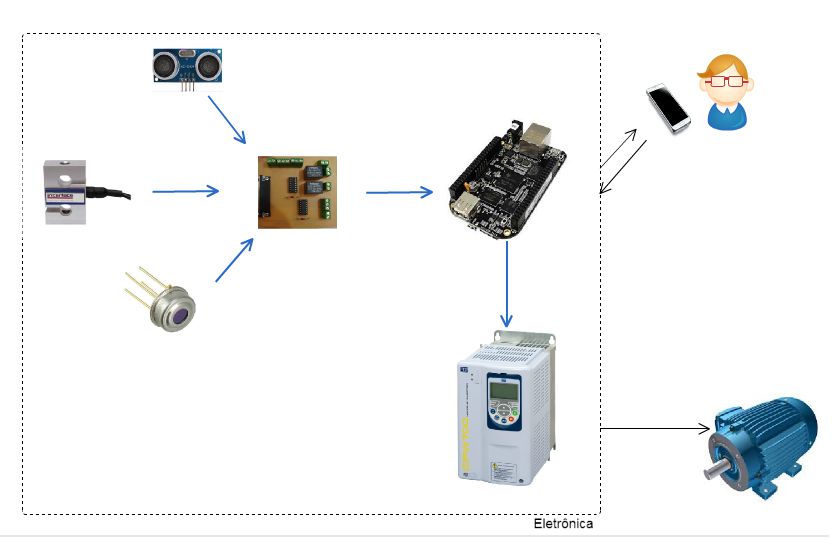
\includegraphics[scale=0.6]{sistema}
		\caption{Sistema proposto simplificado}
		\label{sistema}
	\end{figure}


\subsubsection{Definição da Plataforma de Processamento e Controle}

	Nesse projeto optou-se por utilizar a BeagleBone Black,mostrada na Figura \ref{beaglebone}, que é uma plataforma de desenvolvimento de baixo custo. Segue abaixo alguns dos aspectos que foram levados em consideração para a escolha da mesma.

	\begin{itemize}

		\item Alta capacidade de processamento em comparação às outras plataformas equivalentes, possibilitando a implementação de soluções embarcadas com necessidade de alto desempenho, contém um processador TI Sitara AM3359 ARM Cortex A8 de 1GHz.

		\item Armazenamento on-board de 2Gb,com possibilidade de expansão com microSD, possibilitando maior flexibilidade no desenvolvimento.

		\item Quantidade de pinos GPIOs, especificamente 65, muito superior à quantidade presente em outras plataformas o que trata-se de um fator determinante.

		\item 7 pinos de entrada analógica,com módulos de conversor A/D de 12 bits, capacidade suficiente para interfaceamento com o sistema de sensoriamento.

		\item 8 saídas PWMs, o que é um fator determinante em função da solução adotada para controle de velocidade do motor.

		\item O fato da placa já vir com o sistema Debian previamente instalado facilita no processo de utilização da placa em desenvolvimento em geral.

		\item Possibilidade de suporte por meio da comunidade, visivelmente cada vez mais consolidada.

		\item Grande quantidade de capes desenvolvida pela comunidade BeagleBoard.org, proporcionando redução da complexidade de projeto e implementação do projeto.

	\end{itemize}

	\begin{figure}[!h]
		\centering
		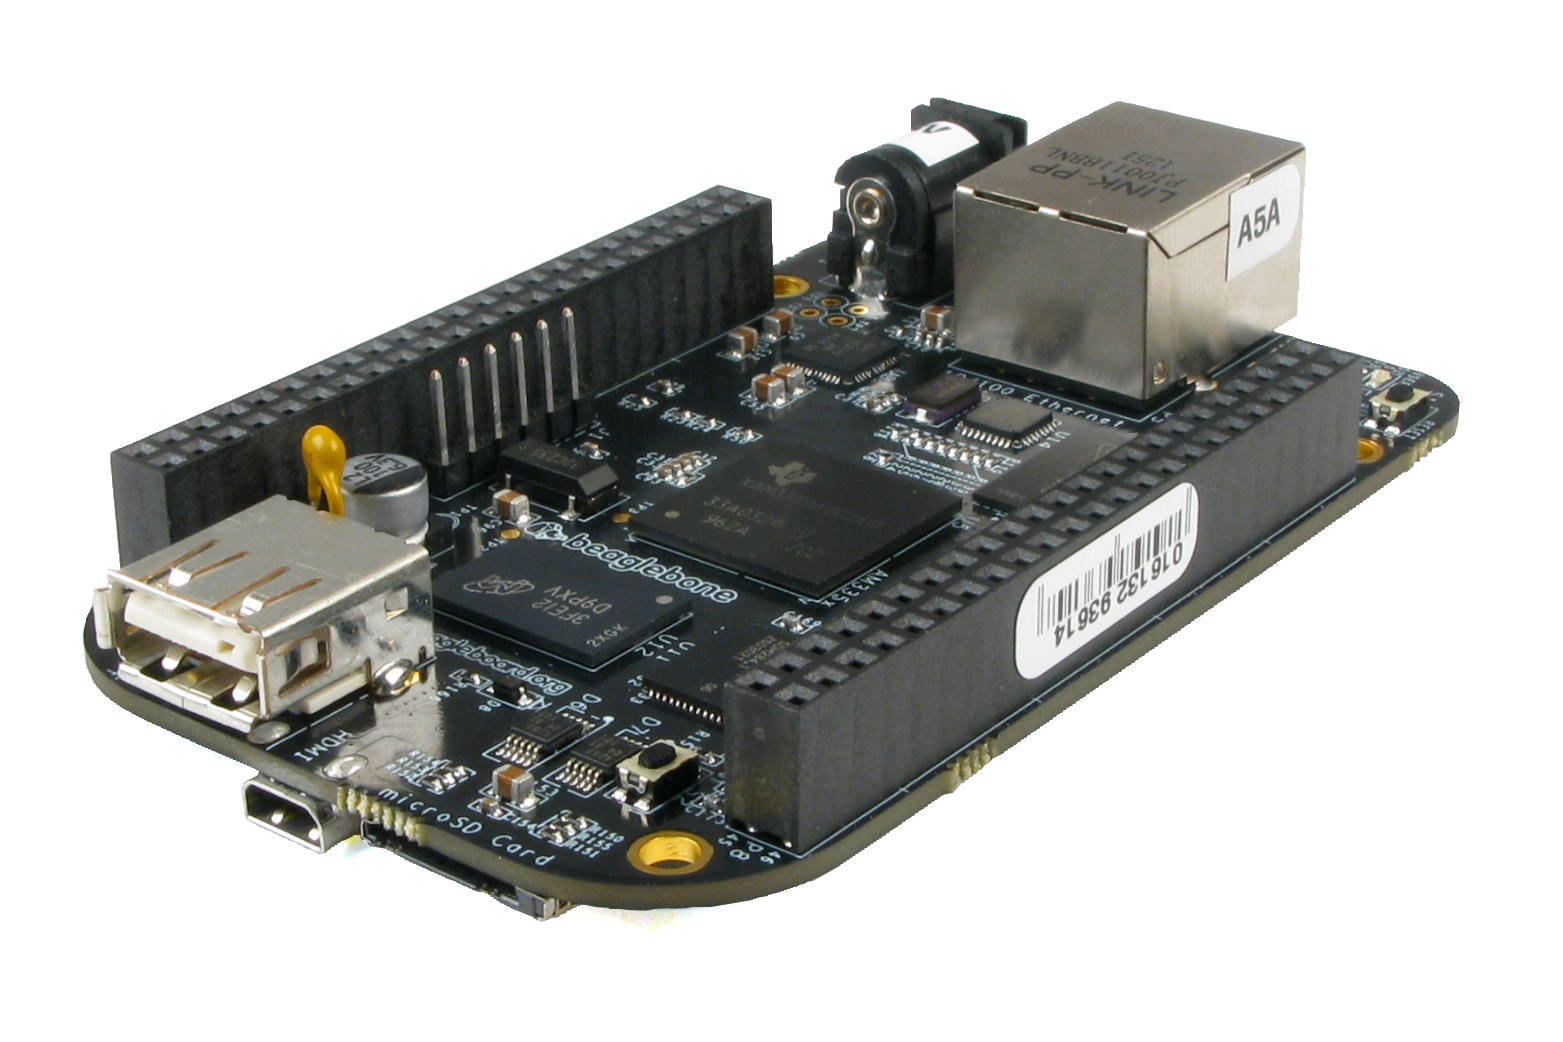
\includegraphics[scale=0.1]{bb.png}
		\caption{BeagleBone Black}
		\label{beaglebone}
	\end{figure}	

\subsubsection{Definição dos sensores}

	Com o objetivo central de obter parâmetros necessários ao processo de caracterização de um amortecedor, a aferição de algumas grandezas torna-se essencial na realização do teste em bancada, os referidos mensuráveis são descritos abaixo:

	\begin{itemize}

		\item Módulo de Velocidade Linear – A resposta de amortecimento é função da velocidade linear da haste, isso porque o aumento da velocidade implica no aumento da absorção de energia do objeto. Optou-se pela utilização de um sensor de proximidade para aferir a posição do amortecedor e em seguida será realizada uma rotina de derivação para obter a velocidade liner do objeto.

		\item Módulo de Força de Reação – Corresponde efetitivamente à saída desejada,com dados referentes à força em diversos contextos de velocidade e temperatura é possível obter os parâmetros de caracterização. Optou-se pela utilização de uma célula de carga em formato S por premitir a aferição de força em movimentos de tração e compressão.

		\item Módulo de Temperatura - A temperatura é um fator essencial no processo de caracterização de um amortecedor em virtude de sua capacidade em alterar o comportamento do mesmo, isso se deve à sensibilidade da viscosidade do fluido à temperatura. Optou-se pela utilização de um sensor de infravermelho em virtude de sua capacidade de aferição da temperatura de um objeto sem contato.

	\end{itemize}

	\subsubsubsection{Módulo de Sensoriamento de Força}

		Segundo o escopo do projeto, a bancada será dimensionada para veículos leves. Comparando-se 3 modelos de veículos leves populares obteve-se os valores de massa máxima, como mostrado na Tabela \ref{comparativocarros}.

		\begin{table}[!h]
		\centering
		\caption{Comparativo de Veículos Leves e Populares}
		%\vspace{0.5cm}
		\begin{tabular}{ l c c c}
		\hline
		\textbf{VEÍCULO/MODELO} & \textbf{PESO BRUTO} & \textbf{PESO EM MARCHA}\\
		\hline
		NOVO UNO VIVACE 1.0 & 1295 Kg & 895 Kg\\
		\hline
		PÁLIO ATTRACTIVE 2014 & 1407 Kg & 1007 Kg\\
		\hline
		NOVO GOL 1.0 TOTAL FLEX & 1387 Kg & 947 Kg\\
		\hline
		\label{comparativocarros}
		\end{tabular}
		\end{table}

			A partir desses três modelos é possível obter um panorama geral para essa classe de veículos em termos de massa. Logo, observa-se que no pior dos casos,especificamente o pálio, dentro desse domínio é a massa de 351Kg em cada amortecedor. Portanto a bancada será projetada para no máximo 400Kg de carga, ou seja para amortecedores de veículos com peso bruto máximo de 1600kg. 
			
			Define-se o formato da célula de carga de acordo com a aplicação, como o carga é sustentada pela célula, é mais indicada a utilização de células em formato de S, por permitirem a aferição de força em movimentos de tração e compressão, além do fato de possuítem capacidade de trabalhar na faixa de valores necessária para o projeto.
			
			Em face dos aspectos apresentados, em uma pesquisa de mercado obteve-se o modelo a ser utilizado no presente projeto, como mostrado na Figura \ref{celuladecarga}
			
		\begin{figure}[!h]
			\centering
			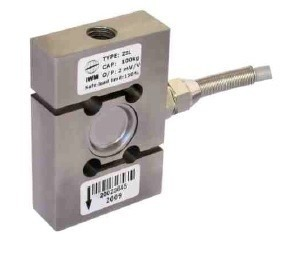
\includegraphics[scale=0.5]{celuladecarga}
			\caption{Célula de Carga - IWM ZSL 500Kg}
			\label{celuladecarga}
		\end{figure}

		Internamente a célula de carga possui uma ponte de Wheatstone responsável por reduzir os ruídos e aumentar a sensibilidade do sistema. Aplica-se uma tensão de referência de 5V e avalia-se a tensão entre os terminais Vs+ e Vs-, a aplicação de uma força implica em uma variação de resistência e consequentemente uma variação de tensão. A variação de tensão, no entanto, é muito baixa,utilizando um amplificador de intrumentação por possui alto ganho, em seguida o sinal é amplificado  que é a tensão máxima permitida nos pinos analógicos da BBB. A Figura \ref{esquematicocelula} apresenta o diagrama de conexão utilizado para a célula de carga.

		\begin{figure}[!h]
			\centering
			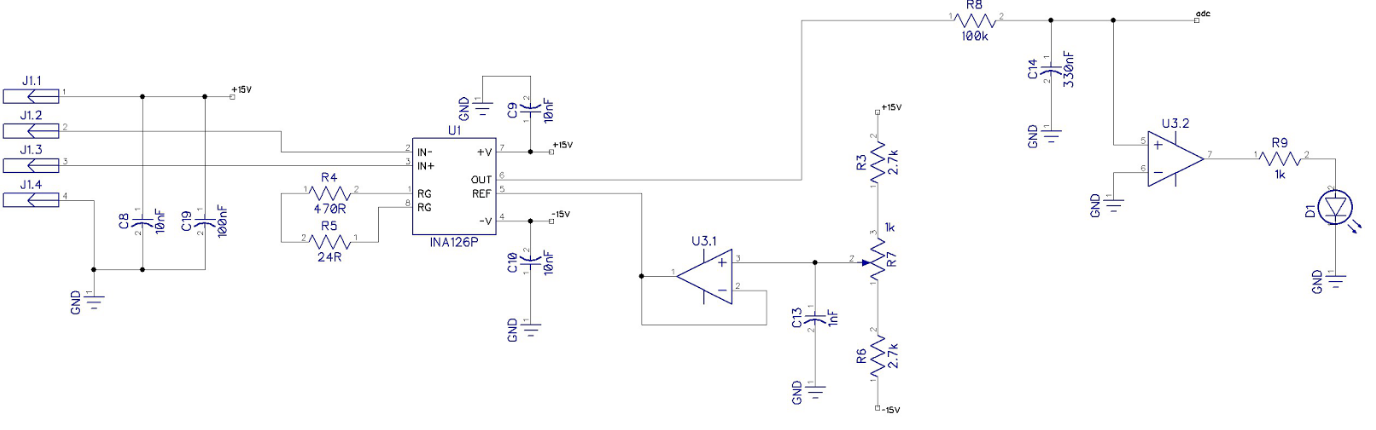
\includegraphics[scale=0.4]{esquematicocelula}
			\caption{Diagrama de Conexão da Célula de Carga}
			\label{esquematicocelula}
		\end{figure}

		Alimentando-se a célula com 5V, e sabendo que o dispositivo possui uma sensibilidade de 2,025mV/V e uma capacidade de 500Kg, conclui-se que a variação de 1Kg implica em uma variação de apenas $20,25\mu V$ por cada Kg. 

		Inicialmente utiliza-se capacitores com o objetivo de contribuir para a anulação do ripple de alta frequência, tornando a alimentação mais estável. Optou-se pela utilização de um INA126 para realizar a amplificação da diferença de potencial medida na célula de carga. 

		Como descrito no datasheet, o componente possui um balanço de zero de 0.0129mV o que significa que na ausência da aplicação de qualquer força a tensão observada será 0.0129, o que trata-se do erro sistemático de medição. Deve-se ajustar a tensão de referência do INA126, utilisou-se uma topologia de comparador de tensão em que é realizada uma comparação entre a saída Vout e a referência, ajusta-se então o potenciômetro, ligado à referência do INA126, até que o LED acenda, tal procedimento deve ser realizado sem carga para se obter a tensão Vout igual a zero para uma carga de 0Kg.

		A BBB possui 7 conversores AD de 12 bits,logo para a faixa de valores de tensão entre 0 e 1.8v obtém-se números discretos entre 0 e 4095. Configurou-se o conversor AD do pino P9\_40 para receber os dados de variação de tensão.

		Segundo informações do datasheet do componente, a curva de sensibilidade pode ser descrita como uma reta com linearidade 0.02\%. Logo, para a faixa de operação do componente, existe uma relação linear entre a força aplicada e a tensão observada. 

		A partir dos dados digitais obtidos implementou-se uma função que relaciona a faixa de valores digitais entre 0 e 4095 e a faixa de valores de medição de carga entre 0 e 500kg.  


	\subsubsubsection{Módulo de Sensoriamento de Velocidade}

		Em virtude da dificuldade de aferição da velocidade linear da haste optou-se pela utilização de um sensor de proximidade e implementar uma função de cálculo da taxa de variação da posição no tempo de amostragem. Em uma pesquisa de mercado optou-se pelo sensor HC-SR04 em virtude da sua fácil aquisição, implementação, faixa de operação larga. A Figura \ref{ultrassom} corresponde ao referido sensor e a  \ref{descricaoHCSR04} aponta algumas de suas principais características.
	
		\begin{figure}[!h]
			\centering
			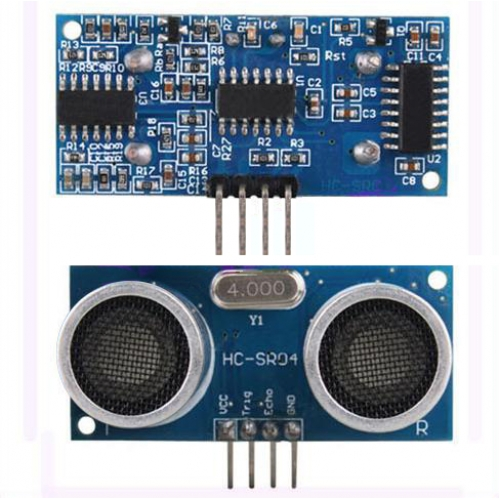
\includegraphics[scale=0.3]{ultrassom.png}
			\caption{Sensor HC-SR04}
			\label{ultrassom}
		\end{figure}

		\begin{table}[!h]
		\centering
		\caption{Características do Sensor HC-SR04}
		\vspace{0.5cm}
		\begin{tabular}{ c c}
		\hline
		\textbf{DESCRIÇÃO}	&	\textbf{VALOR}\\
		\hline
		Tensão de Alimentação DC & 5 V\\
		\hline
		Working Current & 15mA\\
		\hline
		Faixa de Operação & 2cm -  4m\\
		\hline
		Angulo de Medição &  $15^o$\\
		\hline
		Sinal de Trigger de entrada & $10\mu S$ TTL pulso\\
		\hline

		\label{descricaoHCSR04}
		\end{tabular}
		\end{table}

		O princípio de funcionamento do HC-SR04 pode ser entendido analisando-se o seu diagrama de tempo, como mostrado na figura \ref{diagramatempo}

		\begin{figure}[!h]
			\centering
			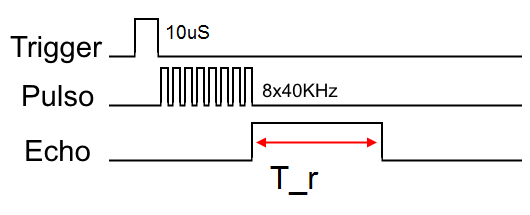
\includegraphics[scale=0.5]{diagrama_tempo_HCSR04.png}
			\caption{Diagrama de tempo do Sensor HC-SR04}
			\label{diagramatempo}
		\end{figure}

		Segundo o datasheet do HC-SR04, para iniciar a medição é necessário enviar um pulso de $10\mu S$ no pino de Trigger, o que corresponde a 8 pulsos de onda sonora visto que a frequência é de 40KHz, o pino de ECHO então fica em nível lógico alto até que seja detectado o sinal da onda refletida pelo objeto, de posse do tempo em que a entrada digital ECHO permanece em nível lógico alto é possível calcular a distância do objeto.

		Como o sistema Linux não é um sistema em tempo real, a utilização desse sensor se torna um pouco complexa em função do princípio de utilização do mesmo. A BBB, no entanto, possui um par de unidades processadoras em tempo real, PRU, ou seja, um par de microcontroladores que operam em uma frequência de 200KHz e permitem que seja executada exatamente uma instrução por ciclo de clock. Com o objetivo de obter precisão nos resultados de temporização dos pulsos de Echo é interessante, portanto, utilizar-se de uma das PRUs disponíveis na BBB.

		Como a BBB recebe um nível de tensão máximo de 3.3V nos seus pinos digitais é necessário adicionar uma topologia de proteção que garanta que o nível de tensão do ECHO do HC-SR04 seja menor que 3.3V. Optou-se pela utilização de um transistor NPN para realizar esse interfaceamento, a Figura \ref{esquematicoHCSR04} apresenta a topologia descrita.

		\begin{figure}[!h]
			\centering
			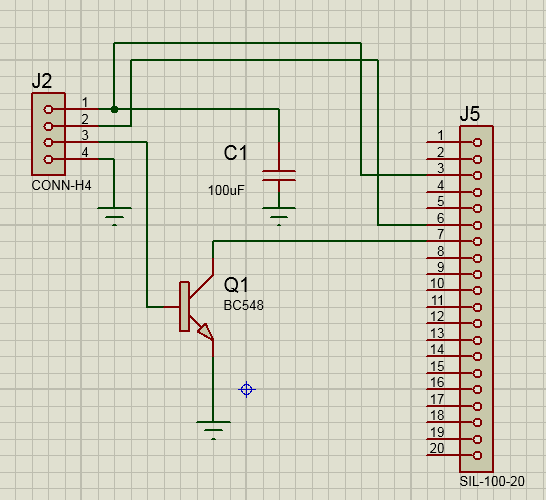
\includegraphics[scale=0.5]{esquematicoHCSR04.png}
			\caption{Diagrama de conexão do HCSR04}
			\label{esquematicoHCSR04}
		\end{figure}


	\subsubsubsection{Módulo de Sensoriamento de Temperatura}

		Em função das características intrínsecas dos testes, optou-se por utilizar sensor com medição sem contato, nesse caso o dispositivo faz uso de tecnologia baseada em sistema infravermelho para realizar a medição. Considerando as condições climáticas do Distrito Federal, amortecedores possuem uma faixa de operação que oscilam em torno de $10^oC \rightarrow 120^oC$. 

		Harmonizando os preceitos apresentados como requisitos do sistema e a questão levantada acima escolheu-se o sensor de temperatura Mlx90614,mostrado na Figura \ref{mlx}, apresenta-se abaixo as principais especificações técnicas do mesmo.

		\begin{figure}[!h]
			\centering
			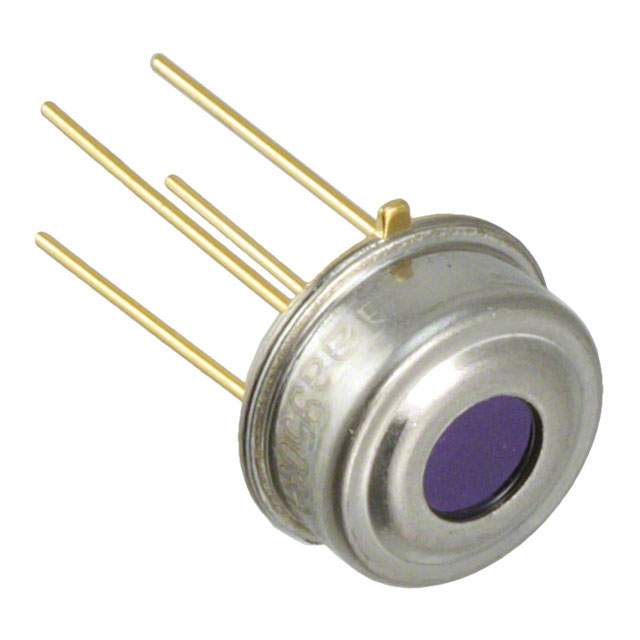
\includegraphics[scale=0.3]{mlx.png}
			\caption{Sensor MLX90614}
			\label{mlx}
		\end{figure}

		O MLX90614 possui uma máquina de estados interna que recebe e calcula a temperatura ambiente e do objeto. O MLX90614 possui a possibilidade de configurar o sinal de saída por PWM ou por interface I2C. No modo PWM o sensor possui uma resolução de $0.14^oC$ e no modo I2C uma resolução de $0.02^oC$, em virtude da melhor resolução optou-se pela utilização no modo I2C. A Figura \ref{esquematicomlx} apresenta a topologia de conexão sugerida pelo datasheet do componente. 

		\begin{figure}[!h]
			\centering
			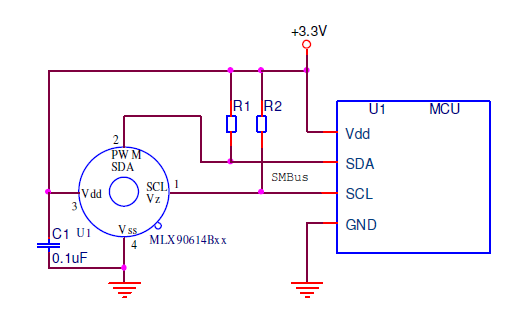
\includegraphics[scale=0.5]{esquematicomlx.png}
			\caption{Diagrama de Conexão do Sensor MLX90614}
			\label{esquematicomlx}
		\end{figure}

		Observa-se que o circuito trata-se de uma topologia com um capacitor de acoplamento e dois resistores de pullup. Em termos de implementação, inicialmente executa-se um parsing responsável por converter a string recebida em base hexadecimal e em seguida realiza a conversão de Kelvins para graus Celsius.
		Os dados de leitura do sensor, temperatura ambiente e temperatura do objeto, são recebidos utilizando interface I2C e armazenados em um vetor de string, o código parcial dessa implementação está disponível no repositório do github.


\subsubsection{PCI de condicionamento dos sinais}

	Como descrito na sessão de sensoriamento, deve-se implementar uma topologia de condicionamento específica para cada sensor, projetou-se uma placa de circuito impresso com o intuito de reduzir os ruídos e, consequentemente, oferecer mais robustez à solução. O esquemático da referida placa é mostrado na Figura \ref{cape}. 

	\begin{figure}[!h]
		\centering
		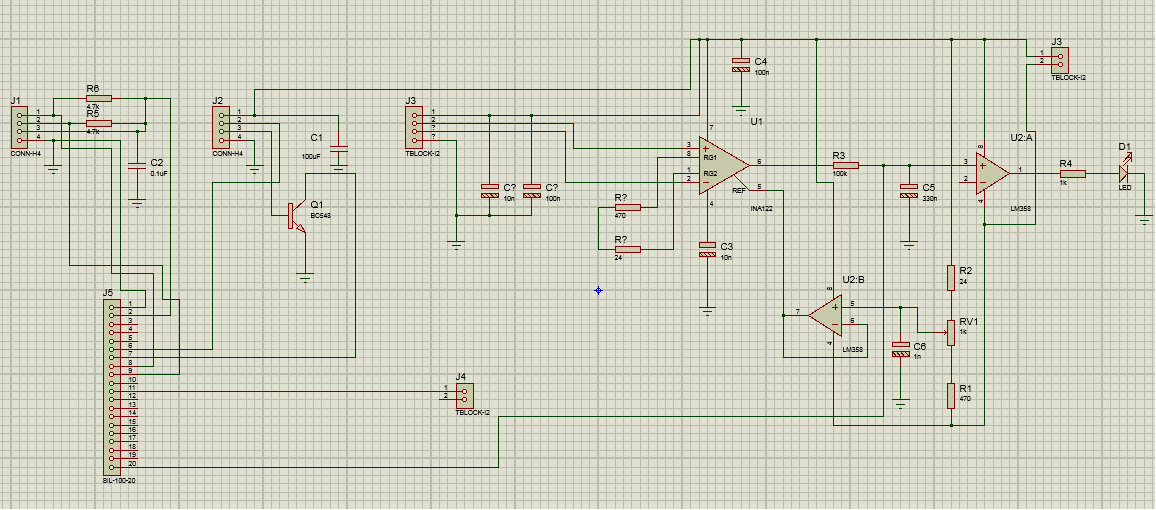
\includegraphics[scale=0.5]{esquematicocape}
		\caption{Esquemático PCI de condicionamento}
		\label{cape}
	\end{figure}

	Como pode ser visto na Figura \ref{cape}, a PCI de condionamento possui os circuitos de condicionamento e os bornes para conexão dos sensores, da porta P9 da BBB da conexão com a entrada analógica do inversor. A Figura \ref{cape3D} mostra uma  visão 3D simulada da placa de condicionamento.

	\begin{figure}[!h]
		\centering
		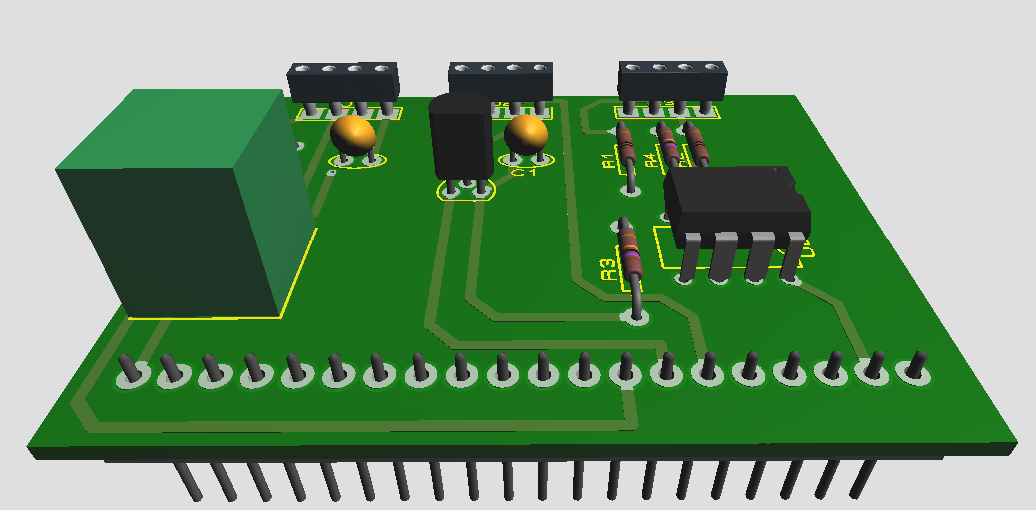
\includegraphics[scale=0.3]{cape3D}
		\caption{Simulação 3D da PCI de Condicionamento}
		\label{cape3D}
	\end{figure}

	A tabela \ref{conexao} apresenta as conexões de cada borne. 

	\newpage
	\begin{table}[!h]
	\centering
	\caption{Tabela de Conexão da PCI de condicionamento}
	%\vspace{0.5cm}
	\begin{tabular}{ c c c }
	\hline
	\textbf{J1 = MLX90614}	& Descrição & Pino BBB\\
	\hline
	1		&	SCL &	P9\_16\\
	\hline
	2		&	SDA &	P9\_18\\
	\hline
	3		&	Vcc &	P9\_4\\
	\hline
	4		&	GND &	P9\_2\\
	\hline
	\textbf{J2 = HC-SR04}	& Descrição & Pino BBB\\
	\hline
	1		&	Vcc &	P9\_6\\
	\hline
	2		&	Trigger &	P9\_12\\
	\hline
	3		&	Echo &	P9\_14\\
	\hline
	4		&	GND &	P9\_2\\
	\hline
	\textbf{J3 = IWM 500Kg}	& Descrição & Pino BBB\\
	\hline
	1		&	Vcc &	P9\_6\\
	\hline
	2		&	Vs+ &	P9\_40\\
	\hline
	3		&	Vs- &	P9\_40\\
	\hline
	4		&	GND &	P9\_2\\
	\hline
	\textbf{J4 = Conexão Inv.}	& Descrição & Pino BBB\\
	\hline
	1		&	S(pwm) &	P9\_22\\
	\hline
	2		&	- &	-\\
	\hline


	\label{conexao}
	\end{tabular}
	\end{table}


	A Tabela \ref{materiais} apresenta a descrição dos componentes necessários à confecção da placa.

	\begin{table}[!h]
	\centering
	\caption{Lista de Componentes}
	\vspace{0.5cm}
	\begin{tabular}{c  c  c  c}
	\hline
	\textbf{Componente} & \textbf{Quantidade} & \textbf{Referência}	& \textbf{Valor}\\
	\hline
	1 &	C1	& 100uF\\
	\hline
	1 &	C2 &	0.1uF\\
	\hline
	2 & C3 e C7 & 10n\\
	\hline
	1 &	C4 &	100n\\
	\hline
	1 &	C5 &	330n\\
	\hline
	1 &	C6 &	1n\\
	\hline
	1 &	D1 &	LED\\
	\hline
	2 &	J1-J2 &	CONN-H4\\
	\hline
	2 &	J3-J4 &	TBLOCK-I2\\
	\hline
	1 &	J5 &	SIL-100-20\\
	\hline
	1 &	Q1 &	BC548\\
	\hline
	2 & R1 e R7 & 470\\
	\hline
	1 &	R2 &	24\\
	\hline
	1 &	R3 &	100k\\
	\hline
	2 & R4 e RV1 & 1k\\
	\hline
	2 &	R5-R6 &	4.7k\\
	\hline
	1 &	U1 &	INA122\\
	\hline
	1 &	U2 &	LM358\\
	\hline

	\label{materiais}
	\end{tabular}
	\end{table}


\subsubsection{Sistema de Controle Embarcado}

	A bancada será controlada por meio de um sistema operacional embarcado na placa beaglebone, usando as técnicas de comunicação TCP/IP para o cliente/servidor, sistema operacional Linux e eletrônica digital para os sensores, como mostrado na Figura \ref{esquema}. O sistema possui as seguintes características:

	\begin{figure}[!h]
		\centering
		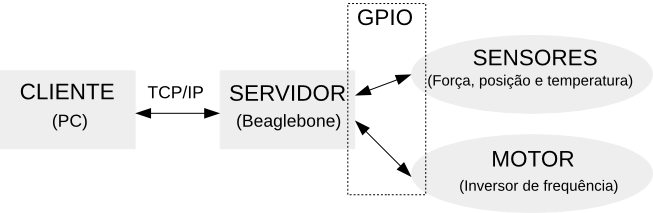
\includegraphics[scale=0.5]{esquemasistemaembarcado.png}
		\caption{Esquema do Sistema Embarcado}
		\label{esquema}
	\end{figure}

	Em um nível mais alto de funcionamento, o sistema deve permitir ao usuário o controle da bancada, com os seguintes comandos: definir parâmetros de teste, iniciar, recuperar dados do último teste, parada de emergência.
	Seguindo as definições de teste apresentadas pela equipe de mecânica, o cliente deve escolher testes em função da velocidade, número de ciclos e temperatura.
	Com isso, o servidor deve receber essas informações e analisá-las, a fim de setar os parâmetros no inversor de frequência, fazendo com que o teste inicie. Durante o ciclo de trabalho, os dados serão salvos e após a conclusão, será enviado para o cliente. É importante ressaltar a importância da integridade desses dados, sendo assim, uma memória extra, não volátil, será usada para salvar os dados e em caso de problemas ou falhas do sistema, os dados experimentais não serão perdidos.
	O sensor de posição determinará o número de ciclos de teste (número de compressão/expansão do pistão do amortecedor. Além disso será usado para obter a velocidade linear desse mesmo eixo.
	Com as informações básicas de funcionamento e tipos de teste a serem realizados, seguem as funcionalidades.


	\textbf{Cliente}\\
	a) Estabelecer conexão:

	Enviar um vetor, sendo a primeira posição o código de estabelecer comunicação e a segunda posição um byte verificador:
		\textit{$Estabelecer comunicação + byte verificador \rightarrow 0xAA + 1 \rightarrow  char = {0xAA, 1}$}
	Após a conexão ser estabelecida com o servidor, ele recebe os dados dos sensores automaticamente, atualizados a cada segundo.

	b) Solicitar teste:

	Cada teste terá um byte verificador único e um código de teste padrão para todos. Além disso, cada teste carrega um tipo de informação relevante, como por exemplo o número de ciclos ou velocidade para o teste. Essas informações devem ser passadas nas posições subsequentes.

		\textit{$Teste + seletor do tipo de teste + parâmetro x + parâmetro y \rightarrow 0xBB + 1 + x + y \rightarrow char[] = {0xBB, 1, x, y}$}
		
	Após a checagem de integridade de pedido pelo servidor, o mesmo retorna os valores dos sensores e informações do inversor de frequência (a fim de ter informações do motor) automaticamente, sendo atualizado a cada segundo.

	c) Backup do último teste:

	Caso os resultados do último teste sejam de interesse do usuário, ele pode solicitar um backup, antes de iniciar o teste atual. Há também um código único para essa opção e um byte verificador.

		\textit{$Backup + byte verificador \rightarrow 0xCC + 1 \rightarrow char[] = {0xCC, 1}$}
		
	d) Encerrar comunicação:

	Após a realização dos testes, o usuário envia ao servidor a informação de encerramento. Isso desconecta o cliente do servidor.

		\textit{$Encerrar + byte verificador \rightarrow 0xDD + 1 \rightarrow char[] = {0xDD, 1}$}
		
	e) Saída de emergência:

	Caso seja necessário interromper o teste por quaisquer motivos, o cliente envia um código de parada de emergência.
		\textit{$Parada de emergência + byte verificador \rightarrow 0xEE + 1 \rightarrow char[] = {0xEE, 1}$}

	\textbf {Servidor}\\
	O servidor aceitará qualquer IP, entretanto, para operar a bancada, será necessário estabelecer a conexão para tal tarefa. As demais informações de tarefa, dado a informação recebida do cliente, segue o padrão descrito para o cliente.

	O sistema operará com o uso de duas treads, uma para cada porta de operação. Uma porta será para todos os testes. A outra é exclusiva para a parada de emergência, que irá ter um sinal de interrupção do sistema, caso seja acionada.

	Os sensores e inversor de frequência serão operados diretamente pelas portas GPIO da placa. Isso significa que esses processos também devem estar rodando em paralelo ao servidor.

	É importante ressaltar que para a construção efetiva sistema cliente/servidor, ou seja, com a determinação exata de quais os parâmetros serão enviados/recebidos, é necessário aguardar as informações da equipe de mecânica. Entretanto a instanciação dos dispositivos na beaglebone, utilizando um cliente/servidor genérico já está sendo implementada. O trabalho já desenvolvido pode ser visualizado no repositório do github:

	\href{https://github.com/ristovao/BancadaDeTesteParaAmortecedor}{https://github.com/ristovao/BancadaDeTesteParaAmortecedor}

\newpage
\subsection{Ponto de Controle III}
\subsubsection{PC III comeca aqui}
	
	TO DO